% 第11章第11节：反复更新的极限与误差（展开递推、谱半径判据、Neumann级数与平衡、收敛速度与暂时放大、逐步误差的累积）。

\section{反复更新的极限与误差}
\label{sec:ls-convergence}
\label{sec:linear-algebra-convergence-approximation}

前两节研究的是一次作用：输入或矩阵有误差时，结果能变化多少。许多计算却反复执行同一个更新：给定实方阵$\bm T\in\mathbb R^{d\times d}$与向量$\bm c\in\mathbb R^d$，从初值$\bm x_0$出发，令
\[
 \bm x_{k+1}=\bm T\bm x_k+\bm c,\qquad k=0,1,2,\ldots
\]
每一轮先对当前状态作同一个线性变换，再加入同一个输入。本节要回答的问题是：无论从哪里出发，这些状态能否趋于同一个平衡？如果能，平衡在哪里，接近得多快，每一轮计算若带有小误差，误差会累积到多大？

我们先展开递推，把状态拆成“初值经过$k$次作用后的剩余影响”与“历次输入的累积”两部分：前者由矩阵幂$\bm T^k$描述，后者由矩阵级数$\sum_j\bm T^j$描述。随后依次研究矩阵幂何时趋于零、矩阵级数收敛到什么、收敛的速度，以及逐步误差的累积。本节只分析给定的$\bm T$与$\bm c$；如何从线性方程出发构造计算便宜且能收敛的更新规则，留给第~\ref{sec:ls-stationary-iterations}节。

本节的收敛按第~\ref{sec:ls-finite-dimensional-sequences}节理解：向量列或矩阵列收敛，等价于每个坐标或每个元素组成的实数列收敛（定理~\ref{thm:multivariable-coordinatewise-convergence}）；由有限维范数等价（定理~\ref{thm:ls-norm-equivalence}），收敛与否不随所选范数改变。所以下面主要在二范数下估计，$\lVert\bm T^k\rVert_2\to0$就是$\bm T^k\to\bm0$。矩阵级数按第~\ref{sec:ls-vector-matrix-series}节的部分和定义收敛，并使用那里的绝对收敛判据。

\subsection{展开递推，分离初值与输入}
\label{sec:ls-affine-iteration-unrolling}

先用一个二维例子看更新规则怎样逐步推进。本节始终用它说明各个结论。
\begin{example}[贯穿本节的更新]
\label{ex:ls-affine-running-example}
给定
\[
 \bm T=\begin{bmatrix}1/2&1\\0&1/2\end{bmatrix},\qquad
 \bm c=\begin{bmatrix}0\\1\end{bmatrix}.
\]
写成分量，更新是$x_{k+1,1}=\tfrac12x_{k,1}+x_{k,2}$与$x_{k+1,2}=\tfrac12x_{k,2}+1$：两个分量每轮各保留一半，第二个分量还把当前值传给第一个分量，随后第二个分量补入$1$。从$\bm x_0=\bm0$出发，
\[
 \bm x_1=\begin{bmatrix}0\\1\end{bmatrix},\quad
 \bm x_2=\begin{bmatrix}1\\3/2\end{bmatrix},\quad
 \bm x_3=\begin{bmatrix}2\\7/4\end{bmatrix}.
\]
例如$\bm x_3=\bm T\bm x_2+\bm c=(\tfrac12+\tfrac32,\tfrac34)^\top+(0,1)^\top$。
\end{example}
三步之后，第二个分量的增量依次为$1/2$、$1/4$，似乎在接近$2$；第一个分量每步增加$1$，看不出是否有界。换一个初值，结果是否相同，也不能由这几步判断。要回答这些问题，先把$\bm x_k$直接写成初值与输入的表达式。

\begin{lemma}[递推的有限展开]
\label{lem:ls-affine-unrolling}
对任意初值$\bm x_0$与$k\geq0$，
\[
 \bm x_k=\bm T^k\bm x_0+\sum_{j=0}^{k-1}\bm T^j\bm c ,
\]
其中$k=0$时和式为空，取为$\bm0$。
\end{lemma}
\begin{proof}
对$k$归纳。$k=0$时两边都是$\bm x_0$。设结论对$k$成立，代入更新规则，
\[
\begin{aligned}
 \bm x_{k+1}&=\bm T\Bigl(\bm T^k\bm x_0+\sum_{j=0}^{k-1}\bm T^j\bm c\Bigr)+\bm c\\
 &=\bm T^{k+1}\bm x_0+\sum_{j=1}^{k}\bm T^j\bm c+\bm T^0\bm c ,
\end{aligned}
\]
这里用了矩阵乘法对加法的分配律，并把和式的指标平移一位。末两项合起来是$\sum_{j=0}^{k}\bm T^j\bm c$，结论对$k+1$成立。
\end{proof}
展开式的第一项$\bm T^k\bm x_0$记录最初状态经过$k$轮作用后的剩余影响。和式中的$\bm T^j\bm c$是$j$轮之前加入的输入再经过$j$次作用的结果，和式把各轮输入的贡献加在一起。$\bm c=\bm0$时，只剩下反复施加同一矩阵的轨迹$\bm T^k\bm x_0$。这里只作了有限展开，还没有假定极限或平衡存在。

比较相同$\bm T,\bm c$而初值不同的两条轨迹$\bm x_k$与$\widetilde{\bm x}_k$。两者的展开式中输入部分相同，相减后只剩
\[
 \bm x_k-\widetilde{\bm x}_k=\bm T^k(\bm x_0-\widetilde{\bm x}_0).
\]
所以“初值是否影响最终结果”只取决于矩阵幂对初始差的作用。只看某一个初始差并不够，下面把“所有初始差都消失”写成关于$\bm T^k$本身的条件。

\begin{lemma}[初值差异消失的条件]
\label{lem:ls-affine-difference-decay}
对固定的$\bm T$与$\bm c$，以下两条等价：
\begin{enumerate}
 \item 对任意两个初值$\bm x_0,\widetilde{\bm x}_0$，相应轨迹满足$\bm x_k-\widetilde{\bm x}_k\to\bm0$；
 \item $\bm T^k\to\bm0$。
\end{enumerate}
\end{lemma}
\begin{proof}
由上式，第一条等价于：对任意$\bm v\in\mathbb R^d$都有$\bm T^k\bm v\to\bm0$。

设$\bm T^k\to\bm0$。按定义$\lVert\bm T^k\rVert_{\mathrm F}\to0$，而二范数不超过Frobenius范数，故对任意$\bm v$，
\[
\begin{aligned}
 \lVert\bm T^k\bm v\rVert_2&\leq\lVert\bm T^k\rVert_2\lVert\bm v\rVert_2\\
 &\leq\lVert\bm T^k\rVert_{\mathrm F}\lVert\bm v\rVert_2\to0 .
\end{aligned}
\]

反过来，设对任意$\bm v$都有$\bm T^k\bm v\to\bm0$。依次取$\bm v=\bm e_1,\ldots,\bm e_d$，$\bm T^k\bm e_j$是$\bm T^k$的第$j$列，所以每一列都趋于零。由定理~\ref{thm:multivariable-coordinatewise-convergence}，每列的各个元素趋于零，于是$\bm T^k$的每个元素趋于零，再由同一定理得$\bm T^k\to\bm0$。
\end{proof}
因此，要判断初值的影响能否全部消失，先研究矩阵幂$\bm T^k$何时趋于零；之后再回到展开式中的输入累积，寻找共同的极限。

\subsection{用谱半径判断初值影响的衰减}
\label{sec:ls-matrix-power-behavior}
\label{sec:linear-algebra-power-convergence}

一个便于检验的充分条件来自范数。若某个次乘性矩阵范数满足$\lVert\bm T\rVert<1$，则$\lVert\bm T^k\rVert\leq\lVert\bm T\rVert^k\to0$，由范数等价即$\bm T^k\to\bm0$。在诱导范数下，这表示每一轮作用都把任何差异缩短到原来的$\lVert\bm T\rVert$倍以内。

贯穿例说明这个条件不必要。$\bm T(0,1)^\top=(1,1/2)^\top$，长度为$\sqrt5/2>1$，所以$\lVert\bm T\rVert_2>1$；由第~\ref{sec:ls-matrix-norms}节的列和与行和公式，$\lVert\bm T\rVert_1=\lVert\bm T\rVert_\infty=3/2$，也都大于$1$。可是示例~\ref{ex:ls-matrix-geometric-series}已经由归纳算出
\[
 \bm T^k=2^{-k}\begin{bmatrix}1&2k\\0&1\end{bmatrix},
\]
由$k2^{-k}\to0$，各元素都趋于零，$\bm T^k\to\bm0$。$\bm T$是上三角矩阵，特征值为对角元$1/2$，谱半径$\rho(\bm T)=1/2$。这个$\bm T$不正规：$\bm T^\top\bm T$的$(1,1)$元为$1/4$，$\bm T\bm T^\top$的$(1,1)$元为$1/4+1=5/4$。对角线上方的耦合使单步放大倍数超过$1$；第~\ref{sec:ls-general-square-spectrum}节已经指出，非正规矩阵的范数可以远大于谱半径。所以需要一个能覆盖非正规矩阵、只依赖谱半径的判据。

下面的引理是这个判据的核心。它先用相似变换把实Schur形的每个对角块化为模长乘旋转，再用逐块的坐标缩放把对角线上方的块压小，构造一个使$\bm T$的诱导范数不超过$r$的坐标范数，从而得到以略大于谱半径的$r$为底的几何上界。为了不与更新矩阵混淆，下面把$\bm T$的实Schur形（定理~\ref{thm:ls-real-schur}）记为$\bm U$。

\begin{lemma}[矩阵幂的几何上界]
\label{lem:ls-power-geometric-bound}
对任意$r>\rho(\bm T)$，存在可逆矩阵$\bm M$，使$\bm T$在坐标范数$\lVert\bm x\rVert_*=\lVert\bm M^{-1}\bm x\rVert_2$诱导的矩阵范数下满足$\lVert\bm T\rVert_*\leq r$；从而存在常数$C_r$，使$\lVert\bm T^k\rVert_2\leq C_rr^k$对所有$k\geq0$成立。
\end{lemma}
\begin{proof}
取实Schur形$\bm T=\bm Q\bm U\bm Q^\top$，其中$\bm Q$正交，$\bm U$分块上三角。设$\bm U$有$s$个对角块，第$i$块的特征值模长为$|\lambda_i|$。

先处理对角块。每个$2\times2$对角块$\bm U_{i,i}$有一对共轭特征值，按第~\ref{sec:ls-general-square-spectrum}节的论证，在复特征向量的实部、虚部组成的基下，它化为模长乘旋转：$\bm U_{i,i}=\bm P_i(|\lambda_i|\bm R_i)\bm P_i^{-1}$，$\bm R_i$为旋转矩阵；$1\times1$块取$\bm P_i=1$、$\bm R_i=\pm1$。

再压小非对角块。对$0<\varepsilon\leq1$，令分块对角矩阵
\[
 \bm D_\varepsilon=\operatorname{diag}(\varepsilon^{0}\bm P_1,\varepsilon^{1}\bm P_2,\ldots,\varepsilon^{s-1}\bm P_s).
\]
直接相乘，$\bm D_\varepsilon^{-1}\bm U\bm D_\varepsilon$的第$(i,j)$块为$\varepsilon^{j-i}\bm P_i^{-1}\bm U_{i,j}\bm P_j$：对角块是$|\lambda_i|\bm R_i$；$j>i$的块带有因子$\varepsilon^{j-i}\leq\varepsilon$，所以全部非对角块组成的矩阵，其Frobenius范数不超过$\varepsilon c$，其中$c$是由各块$\bm P_i^{-1}\bm U_{i,j}\bm P_j$（$j>i$）组成的矩阵的Frobenius范数，与$\varepsilon$无关。把矩阵拆成分块对角部分与非对角部分，得
\[
 \lVert\bm D_\varepsilon^{-1}\bm U\bm D_\varepsilon\rVert_2\leq\rho(\bm T)+\varepsilon c .
\]
这里分块对角部分的二范数不超过$\rho(\bm T)$，是因为把输入按块写成$\bm x=(\bm x_1,\ldots,\bm x_s)$后，输出的平方长度是$\sum_i|\lambda_i|^2\lVert\bm R_i\bm x_i\rVert_2^2\leq\rho(\bm T)^2\lVert\bm x\rVert_2^2$；非对角部分则用二范数不超过Frobenius范数估计。取$\varepsilon$足够小，使右端不超过$r$。

最后构造坐标范数并换回原坐标。令$\bm M=\bm Q\bm D_\varepsilon$，则$\bm M^{-1}\bm T\bm M=\bm D_\varepsilon^{-1}\bm U\bm D_\varepsilon$。$\bm M$可逆，$\lVert\bm x\rVert_*=\lVert\bm M^{-1}\bm x\rVert_2$是一个向量范数：齐次性与三角不等式由$\bm x\mapsto\bm M^{-1}\bm x$的线性和欧氏范数的相应性质得到，而$\lVert\bm x\rVert_*=0$意味着$\bm M^{-1}\bm x=\bm0$，由$\bm M^{-1}$可逆得$\bm x=\bm0$。它就是在新坐标$\bm M^{-1}\bm x$下量取的欧氏长度。令$\bm x=\bm M\bm y$，它诱导的矩阵范数为
\[
\begin{aligned}
 \lVert\bm B\rVert_*
 &=\sup_{\bm x\neq\bm0}\frac{\lVert\bm M^{-1}\bm B\bm x\rVert_2}{\lVert\bm M^{-1}\bm x\rVert_2}\\
 &=\sup_{\bm y\neq\bm0}\frac{\lVert\bm M^{-1}\bm B\bm M\bm y\rVert_2}{\lVert\bm y\rVert_2}
 =\lVert\bm M^{-1}\bm B\bm M\rVert_2 .
\end{aligned}
\]
取$\bm B=\bm T$，得$\lVert\bm T\rVert_*=\lVert\bm D_\varepsilon^{-1}\bm U\bm D_\varepsilon\rVert_2\leq r$。诱导范数满足次乘性，故$\lVert\bm T^k\rVert_*\leq r^k$。再由$\bm T^k=\bm M(\bm M^{-1}\bm T^k\bm M)\bm M^{-1}$及二范数的次乘性，
\[
 \begin{aligned}
 \lVert\bm T^k\rVert_2&\leq\lVert\bm M\rVert_2\lVert\bm M^{-1}\bm T^k\bm M\rVert_2\lVert\bm M^{-1}\rVert_2\\
 &=\lVert\bm M\rVert_2\lVert\bm M^{-1}\rVert_2\lVert\bm T^k\rVert_*\\
 &\leq\lVert\bm M\rVert_2\lVert\bm M^{-1}\rVert_2\,r^k ,
 \end{aligned}
\]
取$C_r=\lVert\bm M\rVert_2\lVert\bm M^{-1}\rVert_2$即可。
\end{proof}
常数$C_r$只依赖固定的换基矩阵$\bm M$，与$k$无关；但$\bm M$随$r$选取，常数也随$r$改变。几何上界也不表示原范数下每一步都收缩：只有在坐标范数$\lVert\cdot\rVert_*$中，$\bm T$的每次作用才不超过$r$倍；换回二范数，单步放大倍数$\lVert\bm T\rVert_2$仍可能大于$1$。下面在贯穿例中具体走一遍这个构造。

\begin{example}[贯穿例的坐标范数]
\label{ex:ls-coordinate-norm-contraction}
贯穿例的$\bm T$已经是上三角矩阵，可取$\bm Q=\bm I$，两个$1\times1$对角块的$\bm P_i=1$，于是$\bm M=\bm D_\varepsilon=\operatorname{diag}(1,\varepsilon)$，且
\[
 \bm M^{-1}\bm T\bm M=\begin{bmatrix}1/2&\varepsilon\\0&1/2\end{bmatrix}.
\]
取$\varepsilon=1/4$。为计算二范数，对$a,b>0$考虑$\bm G=\left[\begin{smallmatrix}a&b\\0&a\end{smallmatrix}\right]$。由式~\eqref{eq:matrix-analysis-spectral-norm}，$\lVert\bm G\rVert_2$是最大奇异值，其平方是$\bm G^\top\bm G=\left[\begin{smallmatrix}a^2&ab\\ab&a^2+b^2\end{smallmatrix}\right]$的最大特征值（第~\ref{sec:ls-svd}节）。这个矩阵的迹为$2a^2+b^2$、行列式为$a^4$，最大特征值为
\[
 \mu=\frac{2a^2+b^2+b\sqrt{b^2+4a^2}}{2}=\Bigl(\frac{b+\sqrt{b^2+4a^2}}{2}\Bigr)^2,
\]
第二个等号展开右端平方即可验证。所以$\lVert\bm G\rVert_2=(b+\sqrt{b^2+4a^2})/2$。代入$a=1/2$、$b=1/4$得
\[
 \lVert\bm T\rVert_*=\frac{1+\sqrt{17}}{8}\approx0.640,
\]
其中$\lVert\bm x\rVert_*=\lVert\bm M^{-1}\bm x\rVert_2=\sqrt{x_1^2+16x_2^2}$。对角矩阵$\operatorname{diag}(d_1,d_2)$满足$\lVert\operatorname{diag}(d_1,d_2)\bm x\rVert_2^2=d_1^2x_1^2+d_2^2x_2^2\leq\max_id_i^2\lVert\bm x\rVert_2^2$，且在相应的标准基向量处取等号，故其二范数为$\max_i|d_i|$。于是$\lVert\bm M\rVert_2=1$、$\lVert\bm M^{-1}\rVert_2=\lVert\operatorname{diag}(1,4)\rVert_2=4$，所以$\lVert\bm T^k\rVert_2\leq4\times0.641^k$。在加大了第二坐标权重的范数中，$\bm T$每一步都收缩；换回欧氏长度，代价是常数$4$。

$r$不能直接取为$\rho(\bm T)=1/2$：由$\bm T^k$的显式式，$\lVert\bm T^k\rVert_2\geq\lVert\bm T^k\bm e_2\rVert_2\geq k2^{1-k}$，即$\lVert\bm T^k\rVert_2/2^{-k}\geq2k$，没有与$k$无关的常数能控制它。
\end{example}

有了几何上界，就能给出矩阵幂衰减的充要条件。
\begin{theorem}[矩阵幂的衰减判据]
\label{thm:ls-power-decay}
对实方阵$\bm T$，$\bm T^k\to\bm0$当且仅当$\rho(\bm T)<1$。
\end{theorem}
\begin{proof}
充分性：取$r$满足$\rho(\bm T)<r<1$。由引理~\ref{lem:ls-power-geometric-bound}，$\lVert\bm T^k\rVert_2\leq C_rr^k$，右端是公比小于$1$的几何数列，趋于零，所以$\bm T^k\to\bm0$。

必要性：设有特征值$|\lambda|\geq1$，要找出一个不趋于零的轨迹。若$\bm T^k\to\bm0$，则对任一固定向量$\bm v$，$\lVert\bm T^k\bm v\rVert_2\leq\lVert\bm T^k\rVert_2\lVert\bm v\rVert_2\to0$。若$\lambda$为实数，取其特征向量$\bm v$，则$\lVert\bm T^k\bm v\rVert_2=|\lambda|^k\lVert\bm v\rVert_2\geq\lVert\bm v\rVert_2$，不趋于零。若$\lambda$非实，取第~\ref{sec:ls-general-square-spectrum}节中对应的二维实不变子空间的基$\bm u,\bm w$，排成列满秩矩阵$\bm P=[\bm u\;\bm w]$；按该节，$\bm T^k\bm P=\bm P|\lambda|^k\bm R^k$，$\bm R$为旋转矩阵。取$\bm P$的左逆$\bm L=(\bm P^\top\bm P)^{-1}\bm P^\top$，则$\bm L\bm T^k\bm u=|\lambda|^k\bm R^k\bm e_1$，其长度为$|\lambda|^k$，所以
\[
 \lVert\bm T^k\bm u\rVert_2\geq\frac{|\lambda|^k}{\lVert\bm L\rVert_2}\geq\frac1{\lVert\bm L\rVert_2}>0,
\]
同样不趋于零。两种情形都有$\bm T^k\not\to\bm0$。
\end{proof}
结合引理~\ref{lem:ls-affine-difference-decay}，所有初值差异都会消失，当且仅当$\rho(\bm T)<1$。判据要求的是全体初值，下面两个例子分别说明，检查一个初始差，或只检查每条轨迹各自收敛，都不足以代替它。

\begin{example}[反例：一个初始差衰减不能说明全部衰减]
\label{ex:ls-partial-convergence}
取$\bm T=\operatorname{diag}(1/2,2)$，比较两个初始差的演化：
\[
\begin{gathered}
\bm T^k\begin{bmatrix}1\\0\end{bmatrix}=\begin{bmatrix}2^{-k}\\0\end{bmatrix}\to\bm0\\
\bm T^k\begin{bmatrix}0\\1\end{bmatrix}=\begin{bmatrix}0\\2^k\end{bmatrix},
\end{gathered}
\]
后者的长度为$2^k\to\infty$。初始差$(1,0)^\top$不含增长方向$\bm e_2$的分量，差异消失；初始差$(0,1)^\top$则被放大。这里$\rho(\bm T)=2>1$。结论：某个特殊初始差衰减，不能说明$\bm T^k\to\bm0$。
\end{example}

\begin{example}[反例：各轨迹收敛但极限不同]
\label{ex:ls-separate-limits}
取$\bm T=\operatorname{diag}(1,1/2)$、$\bm c=\bm0$。对任意初值，
\[
 \bm x_k=\bm T^k\bm x_0=\begin{bmatrix}x_{0,1}\\2^{-k}x_{0,2}\end{bmatrix}\to\begin{bmatrix}x_{0,1}\\0\end{bmatrix}.
\]
每条轨迹都有极限，但极限保留了初值的第一个坐标，不同初值趋于不同的点。这里$\rho(\bm T)=1$，$\bm T^k\to\operatorname{diag}(1,0)\neq\bm0$。结论：各轨迹分别收敛，不等于它们趋于同一极限。
\end{example}

$\rho(\bm T)=1$时，由定理~\ref{thm:ls-power-decay}，$\bm T^k\not\to\bm0$，再由引理~\ref{lem:ls-affine-difference-decay}，初值差异不会全部消失；但不同矩阵的轨迹表现不同，下面看几个例子。仍取$\bm c=\bm0$。$\bm T=\bm I$时$\bm x_k=\bm x_0$，每条轨迹恒定，有界且收敛，但极限就是初值本身；$\bm T=-\bm I$时$\bm x_k=(-1)^k\bm x_0$，非零初值的轨迹来回翻转，有界而不收敛。平面上的$90^\circ$旋转$\bm R=\left[\begin{smallmatrix}0&-1\\1&0\end{smallmatrix}\right]$的特征值为$\pm\mathrm i$，谱半径为$1$；它保持长度，$\lVert\bm R^k\bm x_0\rVert_2=\lVert\bm x_0\rVert_2$，又$\bm R^4=\bm I$而$\bm R\bm x_0\neq\bm x_0$（$\bm x_0\neq\bm0$），所以非零初值的轨迹以$4$步为周期循环，有界而不收敛。下例说明，特征向量不够时还会出现增长。
\begin{example}[反例：谱半径为$1$而矩阵幂无界]
\label{ex:ls-unit-spectral-radius-growth}
给定
\[
 \bm J_1=\begin{bmatrix}1&1\\0&1\end{bmatrix},
\]
它只有特征值$1$，$\rho(\bm J_1)=1$，特征向量只有$(1,0)^\top$的倍数。按示例~\ref{ex:ls-jordan-block-power}的二项式展开，把$0.8$换成$1$，得
\[
 \bm J_1^k=(\bm I+\bm N)^k=\bm I+k\bm N=\begin{bmatrix}1&k\\0&1\end{bmatrix}.
\]
结论：右上角随$k$线性增长，$\lVert\bm J_1^k\rVert_2\geq k\to\infty$；谱半径等于$1$不能保证矩阵幂有界。
\end{example}
这种多项式因子来自对角线上方的耦合。考虑$s$阶矩阵$\bm J=\lambda\bm I+\bm N$，其中$\bm N$是超对角元为$1$、其余元素为零的矩阵，满足$\bm N^s=\bm0$；这样的矩阵称为Jordan块，上例是$\lambda=1$、$s=2$的情形。本节只用这一具体形式，不需要一般的Jordan理论。$\lambda\bm I$与$\bm N$可交换，二项式展开成立，且$j\geq s$的项为零：
\begin{equation}
 \bm J^k=\sum_{j=0}^{\min(k,s-1)}\binom{k}{j}\lambda^{k-j}\bm N^j .
 \label{eq:ch06-jordan-power}
\end{equation}
其中$\binom kj\leq k^j$，$j\leq s-1$。当$s\geq2$、$|\lambda|=1$时，$\bm J^k$的$(1,2)$元为$k\lambda^{k-1}$，模为$k\to\infty$，矩阵幂无界。当$|\lambda|<1$时块幂仍趋于零：$\lambda=0$时$\bm J^k=\bm N^k$在$k\geq s$时为零；$0<|\lambda|<1$时，$\bm J^k$的非零元为$\binom kj\lambda^{k-j}$，模不超过$|\lambda|^{-j}a_k$，其中$a_k=k^j|\lambda|^k$。相邻两项之比$a_{k+1}/a_k=(1+1/k)^j|\lambda|\to|\lambda|<1$；取$q$满足$|\lambda|<q<1$，则$k$充分大后$a_{k+1}\leq qa_k$，$a_k$被一个公比为$q$的几何数列控制，趋于零。不过多项式因子可能使块幂在衰减之前先上升。把上例的特征值从$1$降到$0.8$，就能看到这种先升后降。
\begin{example}[Jordan块幂的先升后降]
\label{ex:ls-jordan-transient}
给定
\[
 \bm J=\begin{bmatrix}0.8&1\\0&0.8\end{bmatrix},
\]
与初值$(0,1)^{\top}$。由示例~\ref{ex:ls-jordan-block-power}，
\[
 \bm J^k\begin{bmatrix}0\\1\end{bmatrix}=\begin{bmatrix}k\,0.8^{k-1}\\0.8^k\end{bmatrix}.
\]
第一坐标在$k=1,2,\ldots,6$时依次为$1$、$1.6$、$1.92$、$2.048$、$2.048$、$1.966$（末项保留三位小数），在$k=4,5$时达到最大值约$2.05$，此后才衰减。结论：特征值$0.8<1$保证最终衰减，但多项式因子$k$使第一坐标先上升到初值长度的两倍以上。
\end{example}
图~\ref{fig:vol1-add-linear-jordan-accumulation}画出这条轨迹的两个坐标。多项式因子也会抬高引理~\ref{lem:ls-power-geometric-bound}中的常数$C_r$。以贯穿例为例，任何对所有$k$满足$\lVert\bm T^k\rVert_2\leq C_rr^k$的常数，都要满足$C_r\geq k2^{1-k}/r^k$对每个$k$成立（示例~\ref{ex:ls-coordinate-norm-contraction}）；固定$k$令$r\downarrow1/2$，右端趋于$2k$。所以$r$越接近$\rho(\bm T)$，可用的常数就必须越大，且没有上界。

\begin{figure}[!htb]
  \centering
  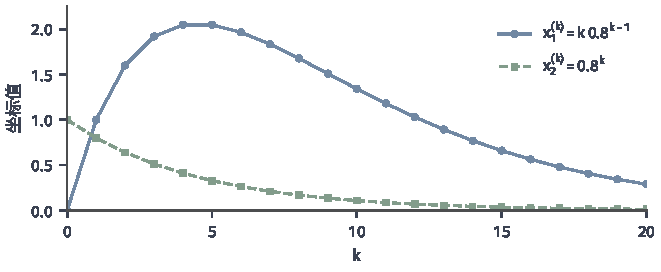
\includegraphics[width=112mm]{figures/00-shared/mathematical-preliminaries-upper/02-linear-spaces/matplotlib/comprehension-additions/linear-jordan-accumulation.pdf}
  \caption{Jordan块的累积项。取正文$\bm J=\left[\begin{smallmatrix}0.8&1\\0&0.8\end{smallmatrix}\right]$与初值$(0,1)^{\top}$。绿线为$0.8^k$，蓝线在$k\geq1$时为$k0.8^{k-1}$，在$k=0$时为$0$。点表示整数步，连线仅引导读图；两坐标最终都趋零。}
  \label{fig:vol1-add-linear-jordan-accumulation}
\end{figure}

$\rho(\bm T)>1$时，由定理~\ref{thm:ls-power-decay}必要性的证明，从模大于$1$的特征值的特征方向（或不变平面）出发的初始差不会消失；但如示例~\ref{ex:ls-partial-convergence}所示，仍可能有特殊初值的差异趋于零。

\subsection{累积输入与共同极限}
\label{sec:ls-matrix-series-exponential}

初值的影响由$\bm T^k$决定，现在回到展开式中的输入累积。若所有轨迹趋于同一个点$\bm x_\star$，在更新规则两边取极限（矩阵乘法是连续的线性作用），它必须满足平衡方程
\[
 \bm x_\star=\bm T\bm x_\star+\bm c ,\quad\text{即}\quad(\bm I-\bm T)\bm x_\star=\bm c .
\]
满足这个方程的点称为更新的平衡点：从它出发，更新不再改变状态。下面的定理说明平衡何时存在唯一，以及何时吸引所有初值。

\begin{theorem}[共同极限的判据]
\label{thm:ls-affine-common-limit}
对固定的$\bm T$与$\bm c$，从任意初值出发的轨迹都收敛到同一个向量，当且仅当$\rho(\bm T)<1$。此时$\bm I-\bm T$可逆，共同极限为$\bm x_\star=(\bm I-\bm T)^{-1}\bm c$，且
\[
 \bm x_k-\bm x_\star=\bm T^k(\bm x_0-\bm x_\star).
\]
\end{theorem}
\begin{proof}
设$\rho(\bm T)<1$。$1$的模不小于$1$，不是$\bm T$的特征值，所以$\det(\bm I-\bm T)\neq0$，$\bm I-\bm T$可逆，平衡方程有唯一解$\bm x_\star=(\bm I-\bm T)^{-1}\bm c$。把$\bm x_{k+1}=\bm T\bm x_k+\bm c$与$\bm x_\star=\bm T\bm x_\star+\bm c$相减，得$\bm x_{k+1}-\bm x_\star=\bm T(\bm x_k-\bm x_\star)$，归纳即得所述等式。由定理~\ref{thm:ls-power-decay}，$\bm T^k\to\bm0$，再由引理~\ref{lem:ls-affine-difference-decay}的证明，$\bm T^k(\bm x_0-\bm x_\star)\to\bm0$，即每条轨迹都收敛到$\bm x_\star$。

反过来，设所有轨迹都收敛到同一个向量$\bm x$。任取两个初值，两条轨迹之差收敛到$\bm x-\bm x=\bm0$。由引理~\ref{lem:ls-affine-difference-decay}，$\bm T^k\to\bm0$，再由定理~\ref{thm:ls-power-decay}，$\rho(\bm T)<1$。
\end{proof}
单有$\bm I-\bm T$可逆，只保证平衡唯一，不保证它吸引其他初值。例如$\bm T=2\bm I$时$\bm I-\bm T=-\bm I$可逆，平衡为$\bm x_\star=-\bm c$，但$\bm x_k-\bm x_\star=2^k(\bm x_0-\bm x_\star)$，除非从平衡出发，轨迹都远离平衡。

定理给出了平衡的位置，但没有说明它怎样由历次输入累积而成。回到有限展开：从$\bm x_0=\bm0$出发，$\bm x_k=\sum_{j=0}^{k-1}\bm T^j\bm c$，正是矩阵级数$\sum_j\bm T^j$的部分和作用在$\bm c$上。按第~\ref{sec:ls-vector-matrix-series}节的定义，矩阵级数$\sum_{j=0}^{\infty}\bm T^j$收敛，指部分和$\bm S_N=\sum_{j=0}^N\bm T^j$作为矩阵序列收敛。对标量$a$，$|a|<1$时几何级数$\sum_ja^j=1/(1-a)$；矩阵情形有同样的结论。

\begin{theorem}[Neumann级数与逆]
\label{thm:ls-neumann}
若$\rho(\bm T)<1$，则级数$\sum_{j=0}^{\infty}\bm T^j$绝对收敛，$\bm I-\bm T$可逆，且
\begin{equation}
 (\bm I-\bm T)^{-1}=\sum_{j=0}^{\infty}\bm T^j .
 \label{eq:ls-neumann-series}
\end{equation}
反之，若这个级数收敛，则$\bm T^k\to\bm0$，从而$\rho(\bm T)<1$。若进一步在某个次乘性矩阵范数下$\lVert\bm T\rVert\leq q<1$，则截断误差满足
\begin{equation}
 \Bigl\lVert(\bm I-\bm T)^{-1}-\sum_{j=0}^{N}\bm T^j\Bigr\rVert\leq\frac{q^{N+1}}{1-q}.
 \label{eq:ls-neumann-tail}
\end{equation}
\end{theorem}
\begin{proof}
先证绝对收敛。取$r$满足$\rho(\bm T)<r<1$，由引理~\ref{lem:ls-power-geometric-bound}，$\lVert\bm T^j\rVert_2\leq C_rr^j$。右端是收敛的标量几何级数的通项，所以$\sum_j\lVert\bm T^j\rVert_2$收敛。由定理~\ref{thm:ls-absolute-series-convergence}，级数$\sum_j\bm T^j$收敛，记其和为$\bm S$，即$\bm S_N\to\bm S$。

再识别级数的和。逐项相消得有限几何和恒等式
\[
 \bm S_N(\bm I-\bm T)=(\bm I-\bm T)\bm S_N=\bm I-\bm T^{N+1}.
\]
令$N\to\infty$。左端是部分和乘以固定矩阵$\bm I-\bm T$。乘以固定矩阵是连续的线性作用（第~\ref{sec:multivariable-continuity}节），具体地，
\[
\begin{aligned}
 &\lVert\bm S_N(\bm I-\bm T)-\bm S(\bm I-\bm T)\rVert_2\\
 &\qquad\leq\lVert\bm S_N-\bm S\rVert_2\lVert\bm I-\bm T\rVert_2\to0 ,
\end{aligned}
\]
左乘同理，所以左端分别收敛到$\bm S(\bm I-\bm T)$与$(\bm I-\bm T)\bm S$；右端由定理~\ref{thm:ls-power-decay}收敛到$\bm I$。极限唯一，故$\bm S(\bm I-\bm T)=(\bm I-\bm T)\bm S=\bm I$，即$\bm I-\bm T$可逆且$(\bm I-\bm T)^{-1}=\bm S$，这就是式~\eqref{eq:ls-neumann-series}。

反过来，若级数收敛，收敛级数的通项趋于零（第~\ref{sec:ls-vector-matrix-series}节）：$\bm T^k=\bm S_k-\bm S_{k-1}\to\bm S-\bm S=\bm0$。再由定理~\ref{thm:ls-power-decay}得$\rho(\bm T)<1$。

最后证截断界。设$\lVert\bm T\rVert\leq q<1$，由次乘性，$\lVert\bm T^j\rVert\leq q^j$，所以级数在这个范数下也绝对收敛。由定理~\ref{thm:ls-absolute-series-convergence}的尾和估计，
\[
 \Bigl\lVert(\bm I-\bm T)^{-1}-\bm S_N\Bigr\rVert
 \leq\sum_{j=N+1}^{\infty}\lVert\bm T^j\rVert
 \leq\sum_{j=N+1}^{\infty}q^j=\frac{q^{N+1}}{1-q},
\]
即式~\eqref{eq:ls-neumann-tail}。
\end{proof}
于是$\rho(\bm T)<1$时，部分和满足$\sum_{j\leq N}\bm T^j\bm c=\bm S_N\bm c$，而$\lVert\bm S_N\bm c-\bm S\bm c\rVert_2\leq\lVert\bm S_N-\bm S\rVert_2\lVert\bm c\rVert_2\to0$，所以
\[
 \bm x_\star=(\bm I-\bm T)^{-1}\bm c=\sum_{j=0}^{\infty}\bm T^j\bm c :
\]
平衡就是全部历次输入经各自轮数传播后的总和。矩阵级数收敛的充要条件也是$\rho(\bm T)<1$。但这一结论针对整个矩阵级数；仅有某一个$\bm c$对应的向量级数$\sum_j\bm T^j\bm c$收敛，推不出同样的结论。例如$\bm T=\operatorname{diag}(1/2,2)$、$\bm c=(1,0)^\top$时，$\sum_j\bm T^j\bm c=(2,0)^\top$收敛，而$\rho(\bm T)=2$。

\begin{example}[贯穿例的平衡]
\label{ex:ls-affine-running-equilibrium}
对示例~\ref{ex:ls-affine-running-example}的更新，平衡方程的第二个分量是$x_{\star,2}=\tfrac12x_{\star,2}+1$，得$x_{\star,2}=2$；第一个分量是$x_{\star,1}=\tfrac12x_{\star,1}+x_{\star,2}$，得$x_{\star,1}=4$。示例~\ref{ex:ls-matrix-geometric-series}已经求出$(\bm I-\bm T)^{-1}=\left[\begin{smallmatrix}2&4\\0&2\end{smallmatrix}\right]$，核对得
\[
 \bm x_\star=\begin{bmatrix}2&4\\0&2\end{bmatrix}\begin{bmatrix}0\\1\end{bmatrix}=\begin{bmatrix}4\\2\end{bmatrix}.
\]
按级数逐项看，$\bm T^j\bm c=2^{-j}(2j,1)^\top$；由示例~\ref{ex:ls-matrix-geometric-series}中的两个标量级数$\sum_j2^{-j}=2$与$\sum_jj\,2^{1-j}=4$，两个分量的和分别为$4$与$2$，与上式一致。结论：开头三步中第一个分量的增长不会无限持续，状态趋于$(4,2)^\top$；由于$\rho(\bm T)=1/2<1$，初值项$\bm T^k\bm x_0$趋于零，从任何初值出发都得到同一个平衡。
\end{example}

Neumann级数定理分开了两种条件。$\rho(\bm T)<1$是级数收敛的充要条件，但只给出定性的收敛；$\lVert\bm T\rVert\leq q<1$是便于检验的充分条件，它给出可以直接计算的截断误差上界。设向量范数与它诱导的矩阵范数满足$\lVert\bm T\rVert\leq q<1$。从$\bm x_0=\bm0$出发，第$k$步只累积到$k-1$次幂，$\bm x_\star-\bm x_k=\bigl((\bm I-\bm T)^{-1}-\bm S_{k-1}\bigr)\bm c$，由式~\eqref{eq:ls-neumann-tail}（取$N=k-1$）与诱导范数的定义，
\[
 \lVert\bm x_k-\bm x_\star\rVert\leq\frac{q^k}{1-q}\lVert\bm c\rVert .
\]
图~\ref{fig:ls-neumann-series-tail}用一个$2\times2$例子核对矩阵尾界。

\begin{figure}[htbp]
 \centering
 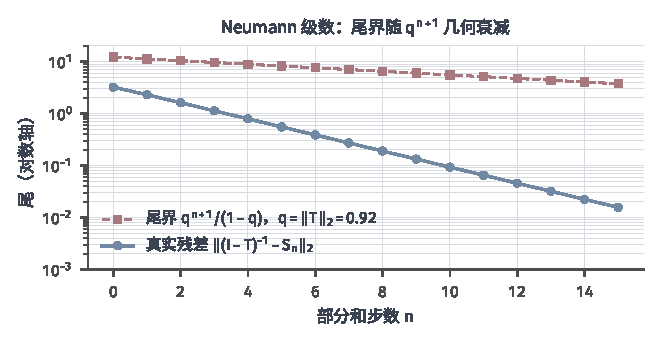
\includegraphics[width=112mm]{figures/00-shared/mathematical-preliminaries-upper/02-linear-spaces/matplotlib/ls-neumann-series-tail/ls-neumann-series-tail.pdf}
 \caption{Neumann级数尾界。$\bm T=[[0.7,0.6],[0,0.1]]$，$q=\lVert\bm T\rVert_2
 \approx0.924<1$，$(\bm I-\bm T)^{-1}=\sum\bm T^k$。蓝线为真实残差
 $\lVert\bm R_n\rVert=\lVert\bm T^{n+1}(\bm I-\bm T)^{-1}\rVert$，红虚线为尾界
 $q^{n+1}/(1-q)$，纵轴半对数（$n=0,\dots,15$）。}
 \label{fig:ls-neumann-series-tail}
\end{figure}

只知道$\rho(\bm T)<1$时，由引理~\ref{lem:ls-power-geometric-bound}，可以取$r<1$并构造坐标范数$\lVert\cdot\rVert_*$，使$\lVert\bm T\rVert_*\leq r$，于是上面的尾界在这个范数中成立。但这个范数依赖换基矩阵$\bm M$；回到原来的误差度量时，须保留比较常数。例如由$\lVert\bm B\rVert_2\leq\lVert\bm M\rVert_2\lVert\bm M^{-1}\rVert_2\lVert\bm B\rVert_*$，二范数下的尾界要再乘以$\lVert\bm M\rVert_2\lVert\bm M^{-1}\rVert_2$。在贯穿例中，示例~\ref{ex:ls-coordinate-norm-contraction}的范数给出$q=(1+\sqrt{17})/8$与$\lVert\bm c\rVert_*=4$；又$\lVert\bm x\rVert_2\leq\sqrt{x_1^2+16x_2^2}=\lVert\bm x\rVert_*$，所以$\lVert\bm x_k-\bm x_\star\rVert_2\leq4q^k/(1-q)\approx11.1\times0.641^k$。例如$k=3$时真实误差$\lVert(2,1/4)^\top\rVert_2\approx2.02$，上界约为$2.92$。

\subsection{收敛速度与暂时放大}
\label{sec:ls-convergence-rate-transient}

谱判据回答了能否收敛，下一个问题是接近平衡有多快。设$\rho(\bm T)<1$，记误差$\bm e_k=\bm x_k-\bm x_\star$。由定理~\ref{thm:ls-affine-common-limit}，$\bm e_k=\bm T^k\bm e_0$；取$\rho(\bm T)<r<1$，由引理~\ref{lem:ls-power-geometric-bound}，
\[
 \lVert\bm e_k\rVert_2\leq C_rr^k\lVert\bm e_0\rVert_2 .
\]
误差至少按略大于谱半径的公比几何衰减。这是对所有初始误差一致成立的上界；某些初始方向的实际误差衰减得更快。例如在贯穿例中，$\bm T\bm e_1=\tfrac12\bm e_1$，取$\bm e_0=\bm e_1$时$\bm e_k=2^{-k}\bm e_1$，每步恰好减半；而下面将看到，从$\bm e_2$出发的误差长度带有因子$2k$。谱半径只决定接近平衡的速度，平衡的位置由$\bm c$与$(\bm I-\bm T)^{-1}$决定。

图~\ref{fig:ls-spectral-radius-convergence}显示最简单的正规情形：误差每步乘以$\rho$，$\rho<1$时衰减，$\rho>1$时增长。

\begin{figure*}[htbp]
 \centering
 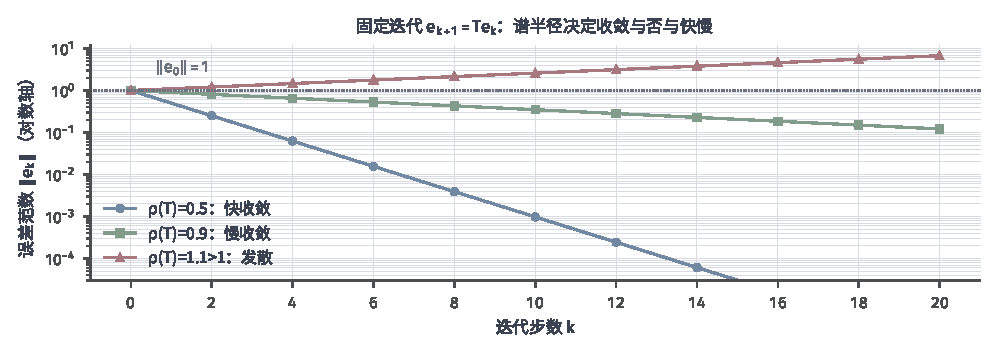
\includegraphics[width=169.0mm]{figures/00-shared/mathematical-preliminaries-upper/02-linear-spaces/matplotlib/ls-spectral-radius-convergence/ls-spectral-radius-convergence.pdf}
 \caption{谱半径决定迭代的长期方向。递推$\bm e^{(t+1)}=\bm A\bm e^{(t)}$、
 $\lVert\bm e^{(0)}\rVert=1$，取正规矩阵$\bm A=\rho\bm I$时$\lVert\bm e^{(t)}\rVert=\rho^t$：
 $\rho=0.5$（蓝）约十四步降到$10^{-4}$，$\rho=0.9$（绿）缓慢下降，
 $\rho=1.1$（红）指数上升。纵轴为半对数。}
 \label{fig:ls-spectral-radius-convergence}
\end{figure*}

上界中的常数$C_r$可能大于$1$，所以长期衰减不排除误差在前几步变大。贯穿例就是这样。
\begin{example}[贯穿例的暂时放大]
\label{ex:ls-running-transient}
在示例~\ref{ex:ls-affine-running-example}中取初值$\bm x_0=\bm x_\star+(0,1)^\top=(4,3)^\top$，即初始误差$\bm e_0=(0,1)^\top$，长度为$1$。由$\bm T^k$的显式式，
\[
 \bm e_k=\bm T^k\bm e_0=2^{-k}\begin{bmatrix}2k\\1\end{bmatrix}.
\]
前三步的误差为$(1,1/2)^\top$、$(1,1/4)^\top$、$(3/4,1/8)^\top$，长度约为$1.118$、$1.031$、$0.760$。结论：前两步的误差都比初始误差长，此后才衰减；谱半径$1/2$只描述长期的衰减速度。
\end{example}
放大来自方向之间的耦合：第二个分量的误差每步把自身传给第一个分量，在第二个分量衰减之前，第一个分量先积累起来。下面的例子耦合更强，放大也更明显。
\begin{example}[非正规矩阵的瞬态放大]
\label{ex:ls-transient-growth}
取$\bm c=\bm0$与另一个更新矩阵$\bm B$，给定
\begin{equation}
\begin{gathered}
\bm B=\begin{bmatrix}0.8&4\\0&0.5\end{bmatrix}\\
\bm x_{k+1}=\bm B\bm x_k\\
\bm x_0=(0,1)^{\top}.
\end{gathered}
\label{eq:ch06-fixed-iteration-example}
\end{equation}
示例~\ref{ex:ls-triangular-power}已把初值沿特征向量$\bm v_1=(1,0)^{\top}$、$\bm v_2=(-40/3,1)^{\top}$分解为$\bm x_0=\tfrac{40}{3}\bm v_1+\bm v_2$，并写出了矩阵幂与轨迹：
\begin{equation}
\begin{gathered}
\bm B^k=
 \begin{bmatrix}
  0.8^k&\frac{40}{3}(0.8^k-0.5^k)\\
  0&0.5^k
 \end{bmatrix}\\
\bm x_k=
 \begin{bmatrix}\frac{40}{3}(0.8^k-0.5^k)\\0.5^k\end{bmatrix}.
\end{gathered}
\label{eq:ch06-diagonalizable-finite-trajectory}
\end{equation}
代入$k=1,2,3$得
\[
 \bm x_1=\begin{bmatrix}4\\0.5\end{bmatrix},\quad
 \bm x_2=\begin{bmatrix}5.2\\0.25\end{bmatrix},\quad
 \bm x_3=\begin{bmatrix}5.16\\0.125\end{bmatrix},
\]
长度分别约为$4.03$、$5.21$、$5.16$，都远大于初值的长度$1$。另一方面$\rho(\bm B)=0.8<1$，由定理~\ref{thm:ls-power-decay}，轨迹最终趋于零。结论：谱半径小于$1$时，轨迹仍可以先放大数倍、再衰减。
\end{example}
放大的原因在于初值沿特征方向的分解。$\tfrac{40}{3}\bm v_1=(40/3,0)^\top$与$\bm v_2=(-40/3,1)^\top$都很长、方向几乎相反，初值$(0,1)^\top$由二者相消而成。两个分量衰减速度不同，相消很快被打破，所以长度先增后降（图~\ref{fig:ch06-transient-growth}）。

\begin{figure*}[htbp]
  \centering
  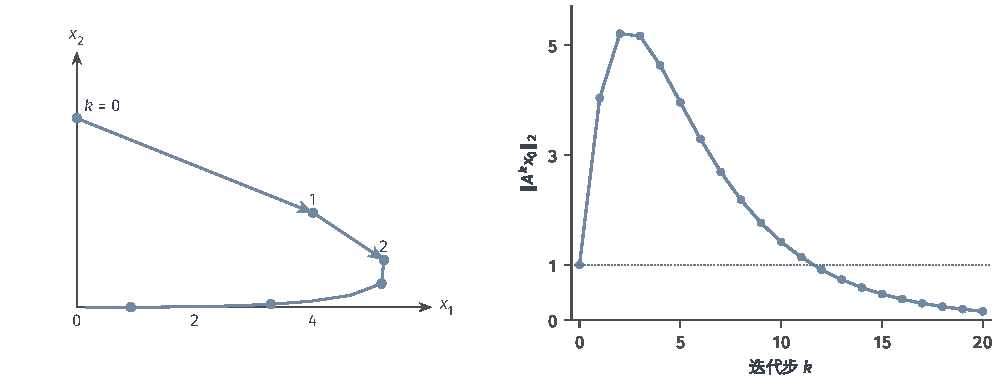
\includegraphics[width=169.0mm]{figures/00-shared/mathematical-preliminaries-upper/02-linear-spaces/matplotlib/ch06-transient-growth/figure.pdf}
  \caption{固定二维矩阵的反复作用。初值为$(0,1)^{\top}$，前两步的长度增加，
  此后回到原点；右图将长度与初始长度$1$比较。特征值$0.8$和$0.5$决定长期衰减，
  非正交特征方向间的相消则决定早期放大。两图使用同一个矩阵和同一组迭代点。}
  \label{fig:ch06-transient-growth}
\end{figure*}

一般地，设$\bm T$能用实可逆矩阵$\bm V$对角化，$\bm T=\bm V\bm\Lambda\bm V^{-1}$，$\bm\Lambda=\operatorname{diag}(\lambda_1,\ldots,\lambda_d)$为实对角矩阵。则$\bm T^k=\bm V\bm\Lambda^k\bm V^{-1}$；又$\lVert\bm\Lambda^k\bm x\rVert_2^2=\sum_i\lambda_i^{2k}x_i^2\leq\rho(\bm T)^{2k}\lVert\bm x\rVert_2^2$，即$\lVert\bm\Lambda^k\rVert_2\leq\rho(\bm T)^k$。由次乘性，
\[
 \lVert\bm T^k\rVert_2\leq\lVert\bm V\rVert_2\lVert\bm V^{-1}\rVert_2\,\rho(\bm T)^k .
\]
因子$\lVert\bm V\rVert_2\lVert\bm V^{-1}\rVert_2$不小于$1$，因为$1=\lVert\bm V\bm V^{-1}\rVert_2\leq\lVert\bm V\rVert_2\lVert\bm V^{-1}\rVert_2$；它越大，这个上界允许的早期放大越强。在示例~\ref{ex:ls-transient-growth}中取$\bm V=[\bm v_1\;\bm v_2]$，两条特征方向的夹角只有约$4.3^\circ$（示例~\ref{ex:ls-nonnormal-norm-radius}）。直接验证$\bm V^{-1}=\left[\begin{smallmatrix}1&40/3\\0&1\end{smallmatrix}\right]$，于是$\lVert\bm V\rVert_2\geq\lVert\bm V\bm e_2\rVert_2=\lVert\bm v_2\rVert_2\approx13.37$，$\lVert\bm V^{-1}\rVert_2\geq\lVert\bm V^{-1}\bm e_2\rVert_2\approx13.37$，乘积超过$178$。

贯穿例与示例~\ref{ex:ls-jordan-transient}则不可对角化。以贯穿例为例，它只有特征值$1/2$，而$\bm T-\tfrac12\bm I=\left[\begin{smallmatrix}0&1\\0&0\end{smallmatrix}\right]$的零空间只是$\operatorname{span}\{\bm e_1\}$，凑不出两个线性无关的特征向量；两例的放大都来自式~\eqref{eq:ch06-jordan-power}中的多项式因子。正规矩阵与此相反：第~\ref{sec:ls-general-square-spectrum}节证明了$\lVert\bm T^k\rVert_2=\rho(\bm T)^k$，每一步的最大放大倍数恰为谱半径。其中幂次取$1$得$\lVert\bm T\rVert_2=\rho(\bm T)$，于是每一步都有$\lVert\bm e_{j+1}\rVert_2\leq\lVert\bm T\rVert_2\lVert\bm e_j\rVert_2=\rho(\bm T)\lVert\bm e_j\rVert_2$，所以$\rho(\bm T)<1$时误差的长度从第一步起就不增加。所以，长期衰减、有限步内的最大放大和具体初始方向的表现要分别考察，不能只用谱半径估计中途的误差。

暂时放大说明谱半径不是单步倍率。它确切刻画的是矩阵幂的长期几何速率。
\begin{theorem}[Gelfand公式]
\label{thm:ls-gelfand-formula}
对实方阵$\bm T$与$d\times d$矩阵空间上的任意范数$\lVert\cdot\rVert$，
\begin{equation}
 \rho(\bm T)=\lim_{k\to\infty}\lVert\bm T^k\rVert^{1/k}.
 \label{eq:ls-gelfand-formula}
\end{equation}
若该范数还满足次乘性，则$\rho(\bm T)\leq\lVert\bm T\rVert$。
\end{theorem}
\begin{proof}
先在二范数中证明。上界：对任意$r>\rho(\bm T)$，由引理~\ref{lem:ls-power-geometric-bound}，$\lVert\bm T^k\rVert_2^{1/k}\leq C_r^{1/k}r$，而$C_r^{1/k}\to1$，所以$\limsup_k\lVert\bm T^k\rVert_2^{1/k}\leq r$。

下界：取模为$\rho(\bm T)$的特征值$\lambda$，重复定理~\ref{thm:ls-power-decay}必要性证明中的估计。若$\lambda$为实数，取单位特征向量$\bm v$，则$\lVert\bm T^k\rVert_2\geq\lVert\bm T^k\bm v\rVert_2=\rho(\bm T)^k$。若$\lambda$非实，同一证明中的$\bm u\neq\bm0$满足$\lVert\bm T^k\bm u\rVert_2\geq\rho(\bm T)^k/\lVert\bm L\rVert_2$，所以$\lVert\bm T^k\rVert_2\geq c\,\rho(\bm T)^k$，其中$c=1/(\lVert\bm L\rVert_2\lVert\bm u\rVert_2)>0$与$k$无关。两种情形都有$\lVert\bm T^k\rVert_2^{1/k}\geq c^{1/k}\rho(\bm T)$（实特征值时$c=1$），而$c^{1/k}\to1$，故$\liminf_k\lVert\bm T^k\rVert_2^{1/k}\geq\rho(\bm T)$。

合起来，$\rho(\bm T)\leq\liminf_k\lVert\bm T^k\rVert_2^{1/k}\leq\limsup_k\lVert\bm T^k\rVert_2^{1/k}\leq r$对每个$r>\rho(\bm T)$成立。令$r$趋于$\rho(\bm T)$，上下极限相等，极限存在且等于$\rho(\bm T)$。

再推广到任意范数。由有限维范数等价（定理~\ref{thm:ls-norm-equivalence}），存在与矩阵无关的常数$0<c_1\leq c_2$，使$c_1\lVert\bm B\rVert_2\leq\lVert\bm B\rVert\leq c_2\lVert\bm B\rVert_2$对所有$d$阶方阵成立。取$\bm B=\bm T^k$并开$k$次方，$c_1^{1/k}$与$c_2^{1/k}$都趋于$1$，由夹逼，$\lVert\bm T^k\rVert^{1/k}$与$\lVert\bm T^k\rVert_2^{1/k}$有相同的极限。

最后，若范数满足次乘性，则$\lVert\bm T^k\rVert\leq\lVert\bm T\rVert^k$，即$\lVert\bm T^k\rVert^{1/k}\leq\lVert\bm T\rVert$对每个$k$成立。令$k\to\infty$即得$\rho(\bm T)\leq\lVert\bm T\rVert$。
\end{proof}
最后一条说明，次乘性范数小于$1$必定使谱半径小于$1$，这正是本节开头的充分条件；贯穿例说明反过来不成立。Gelfand公式说明，谱半径是矩阵幂最大放大倍数的长期几何平均。它不表示每条误差轨迹每一步都乘以同一个倍率：某些初值可能不含最慢衰减方向，非正规作用还可能在早期放大误差。

设$0<\rho(\bm T)<1$。若粗略用$\rho(\bm T)^m$估计$m$步后的长期倍率，由$\rho(\bm T)^m=1/10$得到缩小十倍的参考步数
\[
 m=\frac{1}{\log_{10}\bigl(1/\rho(\bm T)\bigr)} .
\]
例如$\rho=0.5$时约为$3.3$步，$\rho=0.99$时约为$229$步：谱半径接近零时每步都显著缩小误差，接近一时缩小十倍要上百步。实际达到给定精度的步数还受常数、初始方向和暂时放大的影响。在示例~\ref{ex:ls-running-transient}中，参考步数约为$3.3$，但$\lVert\bm e_k\rVert_2=2^{-k}\sqrt{4k^2+1}$在$k=1,\ldots,7$时依次约为$1.118$、$1.031$、$0.760$、$0.504$、$0.314$、$0.188$、$0.110$，到$k=8$才第一次降到$0.1$以下（约为$0.063$），即要$8$步才缩小十倍。精确解未知时还需要用可计算的量判断何时停止，这在第~\ref{sec:ls-stationary-iterations}节联系残差讨论。

\subsection{逐步误差的累积}
\label{sec:ls-accumulated-step-errors}

前面假设每一轮都精确执行。实际计算中，每轮可能引入新的误差，例如舍入，或者只近似地算出$\bm T\bm y_k$。把第$k$轮附加的误差记为$\bm\delta_k$，实际得到的序列满足
\[
 \bm y_{k+1}=\bm T\bm y_k+\bm c+\bm\delta_k .
\]
设$\rho(\bm T)<1$，$\bm x_\star$为定理~\ref{thm:ls-affine-common-limit}中的平衡，令$\bm e_k=\bm y_k-\bm x_\star$。与$\bm x_\star=\bm T\bm x_\star+\bm c$相减，得$\bm e_{k+1}=\bm T\bm e_k+\bm\delta_k$。这与开头的更新形式相同，只是每轮的输入换成了$\bm\delta_k$，于是可以仿照有限展开分析。

\begin{theorem}[逐步误差的累积]
\label{thm:ls-accumulated-step-errors}
设$\rho(\bm T)<1$，$\bm y_k$与$\bm e_k$如上。
\begin{enumerate}
 \item 对每个$k\geq0$，
 \[
  \bm e_k=\bm T^k\bm e_0+\sum_{j=0}^{k-1}\bm T^{k-1-j}\bm\delta_j .
 \]
 \item 取一个向量范数及其诱导的矩阵范数，若$\lVert\bm T\rVert\leq q<1$且$\lVert\bm\delta_j\rVert\leq\delta$对所有$j$成立，则
 \begin{equation}
  \lVert\bm e_k\rVert\leq q^k\lVert\bm e_0\rVert+\delta\,\frac{1-q^k}{1-q},
  \label{eq:ls-noise-floor}
 \end{equation}
 从而$\limsup_{k\to\infty}\lVert\bm e_k\rVert\leq\delta/(1-q)$。
 \item 若只知道$\rho(\bm T)<1$，取$\rho(\bm T)<r<1$与引理~\ref{lem:ls-power-geometric-bound}中的常数$C_r$。若$\lVert\bm\delta_j\rVert_2\leq\delta$对所有$j$成立，则
 \[
  \lVert\bm e_k\rVert_2\leq C_rr^k\lVert\bm e_0\rVert_2+C_r\delta\,\frac{1-r^k}{1-r}.
 \]
\end{enumerate}
\end{theorem}
\begin{proof}
第一条对$k$归纳。$k=0$时和式为空。设等式对$k$成立，则
\[
\begin{aligned}
 \bm e_{k+1}&=\bm T\bm e_k+\bm\delta_k\\
 &=\bm T^{k+1}\bm e_0+\sum_{j=0}^{k-1}\bm T^{k-j}\bm\delta_j+\bm T^0\bm\delta_k ,
\end{aligned}
\]
末两项合起来是$\sum_{j=0}^{k}\bm T^{k-j}\bm\delta_j$，即$k+1$时的等式。

第二条。由三角不等式、诱导范数的界与次乘性，$\lVert\bm T^i\bm v\rVert\leq q^i\lVert\bm v\rVert$，所以
\[
\begin{aligned}
 \lVert\bm e_k\rVert&\leq q^k\lVert\bm e_0\rVert+\sum_{j=0}^{k-1}q^{k-1-j}\delta\\
 &=q^k\lVert\bm e_0\rVert+\delta\sum_{i=0}^{k-1}q^i ,
\end{aligned}
\]
末项的有限几何和等于$\delta(1-q^k)/(1-q)$，这就是式~\eqref{eq:ls-noise-floor}。右端随$k\to\infty$收敛到$\delta/(1-q)$，所以$\lVert\bm e_k\rVert$的上极限不超过它。

第三条。把第一条的展开取二范数，用$\lVert\bm T^i\rVert_2\leq C_rr^i$代替第二条中的$q^i$，同样求和即得。
\end{proof}
展开式中，第一项是初始误差的传播，按几何速度消失；和式中，$j$轮的附加误差再经过$k-1-j$次作用，较早的误差衰减得多，较近的误差几乎原样保留。所以持续的附加误差不会随迭代消失，式~\eqref{eq:ls-noise-floor}右端随$k$增大趋于$\delta/(1-q)$，$q$越接近$1$，这个上界越大。

这是持续有界扰动下的最坏情形上界。它不是每条轨迹必然达到的误差下限：例如各轮误差都为零时，$\bm e_k=\bm T^k\bm e_0\to\bm0$，最终远小于$\delta/(1-q)$。它也不保证误差存在极限。取$\bm T=\bm0$、$\bm c=\bm0$，则$\bm x_\star=\bm0$、$q=0$；再取单位向量$\bm u$与交替变号的附加误差$\bm\delta_k=(-1)^k\delta\bm u$，则$\bm e_k=\bm\delta_{k-1}=(-1)^{k-1}\delta\bm u$（$k\geq1$）。误差的长度始终等于上界$\delta/(1-q)=\delta$，说明这个上界不能再改进，但$\bm e_k$来回翻转，没有极限。

第三条中两项都带着常数$C_r$：在非正规的$\bm T$下，即使每轮附加的误差很小，它们在被衰减之前也可能先被暂时放大，累积的上界因此按$C_r$倍增大。本节假设$\bm T$固定；具体算法如何产生附加误差、怎样选择更新规则和参数、何时停止计算，留给第~\ref{sec:ls-stationary-iterations}节处理。
